\chapter{Caracterización del  Electroimán} \chapterlabel{Informe/3-CaracterizaciónElectroimán} \label{cap:CaracterizaciónElectroimán}

\section{Caracterización del Electroimán}

El actuador de este sistema de control es un electroimán. Se eligió construirlo utilizando un núcleo de acero al silicio con un bobinado en su interior. 
%mejorar esto

Se puede modelar el problema como un objeto de masa puntual que es sometido a dos fuerzas opuestas en el eje “Y” de la figura \ref{fig:img_modelado-fisico}: la de su propio peso hacia abajo, y una fuerza realizada por el electroimán en sentido contrario.

%capaz poner otra imagen
\begin{figure}[H]
	\centering
	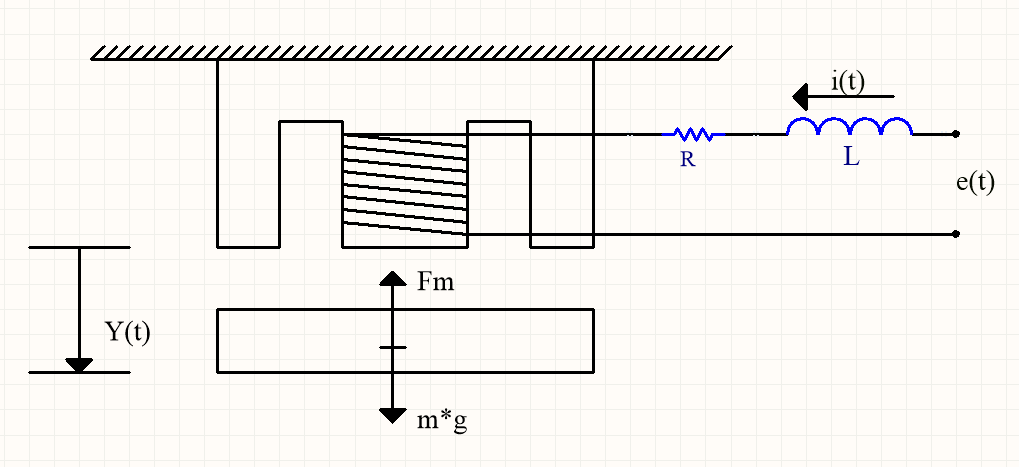
\includegraphics[width=\textwidth]{modelo-fisico.png}
	\caption{Modelado físico.}
	\label{fig:img_modelado-fisico}
\end{figure}

Se sabe que la fuerza correspondiente al peso del objeto es $F_{m}=m*g$. Por lo tanto, el electroimán debe generar una fuerza de igual módulo y sentido contrario para mantenerlo suspendido en estado de equilibrio. Esta fuerza se obtiene de la circulación de un flujo magnético entre el núcleo del electroimán y la pieza con forma de I. Para generar el flujo magnético se necesita una fuerza magnetomotriz.

%esto es otra cosa ya. hacer una intro de como se genera la fuerza magnética???
La fuerza magnetomotriz generada en el núcleo del electroimán es proporcional a la corriente que circula por su bobinado, y su módulo está dado por la ecuación \ref{eq_fuerza-magnetomotriz}. Para poder modelarla se debe realizar un análisis físico del actuador. 

\begin{equation} \label{eq_fuerza-magnetomotriz}
	F_{mm}=R_{m}*\phi=N*i	
\end{equation}

%mejorar este parrafo
En donde $R_{m}$ corresponde a la reluctancia del circuito magnético, $\phi$ indica la magnitud del flujo, es decir, la cantidad de campo magnético que atravies una superficie y $F_{mm}$ es la fuerza magnetomotriz (que es distinta a la fuerza magnética $F_{m}$). La ley de Hopkinson relaciona estos parámetros con la corriente que circula por el bobinado ($i$) y la cantidad de vueltas de su núcleo ($N$).


Por otro lado, la inductancia del bobinado está dada por la ecuación \ref{eq_inductancia_flujo}

\begin{equation} \label{eq_inductancia_flujo}
	L*i=N*\phi
\end{equation}


Como se ve en la figura \ref{fig:img_modelado-fisico}, el electroimán utilizado está compuesto por una pieza en forma de E y otra en forma de I, que se encuentran separadas por un espacio o gap de aire. Este circuito magnético se puede modelar como a un toroide con un corte o separación  de longitud $lA=2*y$, como se muestra en la figura \ref{fig:img_toroide}

\begin{figure}[H]
	\centering
	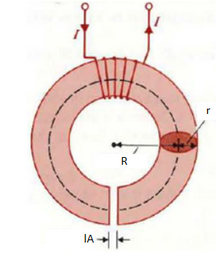
\includegraphics[scale=0.75]{toroide.png}
	\caption{Toroide con gap de aire.}
	\label{fig:img_toroide}
\end{figure}

Para el análisis se utiliza la ecuación qwf para modelar la reluctancia de un toroide sin gap de aire, con área transversal A y longitud del circuito magnético $l_{h}$. 

\begin{equation}\label{eq_reluctancia}
	R_{m}=\frac{l_{h}}{\mu_{o}*\mu_{r}*A}
\end{equation}

a
a
a
a


En la Figura 3.1 se puede observar una representación física del problema.


A partir del modelado físico del electroimán se llega a la expresión de la inductancia (L) en función del gap de aire (Y) (ecuación 3.1) y de la fuerza magnética ejercida por el electroimán (Fm) (ecuación 3.2):


